%%% LaTeX Template: Two column article
%%%
%%% Source: http://www.howtotex.com/
%%% Feel free to distribute this template, but please keep to referal to http://www.howtotex.com/ here.
%%% Date: February 2011

%%% Preamble
\documentclass[	DIV=calc,%
							paper=a4,%
							fontsize=12pt,%
							onecolumn]{scrartcl}	 					% KOMA-article class

\usepackage{lipsum}													% Package to create dummy text
\usepackage[brazil]{babel}										% English language/hyphenation
\usepackage[protrusion=true,expansion=true]{microtype}				% Better typography
\usepackage{amsmath,amsfonts,amsthm}					% Math packages
\usepackage[pdftex]{graphicx}									% Enable pdflatex
\usepackage[svgnames]{xcolor}									% Enabling colors by their 'svgnames'
\usepackage[hang, small,labelfont=bf,up,textfont=it,up]{caption}	% Custom captions under/above floats
\usepackage{epstopdf}											% Converts .eps to .pdf
\usepackage{subfig}													% Subfigures
\usepackage[pdftex]{hyperref}
\usepackage{booktabs}												% Nicer tables
\usepackage{fix-cm}													% Custom fontsizes
\usepackage[utf8]{inputenc}
\usepackage[top=2.5cm, bottom=2.5cm, left=2.5cm, right=2.5cm]{geometry}
\usepackage[ddmmyyyy]{datetime}
\addto\captionsenglish{%
	\renewcommand\tablename{Tabela}
	\renewcommand\figurename{Figura}
} 
 

 
%%% Custom sectioning (sectsty package)
\usepackage{sectsty}													% Custom sectioning (see below)
\allsectionsfont{%															% Change font of al section commands
	\usefont{OT1}{phv}{b}{n}%										% bch-b-n: CharterBT-Bold font
	}

\sectionfont{%																% Change font of \section command
	\usefont{OT1}{phv}{b}{n}%										% bch-b-n: CharterBT-Bold font
	}

\usepackage{float} % here for H placement parameter


%%% Headers and footers
\usepackage{fancyhdr}												% Needed to define custom headers/footers
	\pagestyle{fancy}														% Enabling the custom headers/footers
\usepackage{lastpage}	

% Header (empty)
\lhead{}
\chead{}
\rhead{}
% Footer (you may change this to your own needs)

%% ====================================
%% ====================================
%% mude o rodape  do projeto
%% ====================================
%% ====================================

\lfoot{\footnotesize \texttt{Template para entrega de texto} \textbullet ~Modelo de projeto}


\cfoot{}
\rfoot{\footnotesize página \thepage\ de \pageref{LastPage}}	% "Page 1 of 2"
\renewcommand{\headrulewidth}{0.0pt}
\renewcommand{\footrulewidth}{0.4pt}



%%% Creating an initial of the very first character of the content
\usepackage{lettrine}
\newcommand{\initial}[1]{%
     \lettrine[lines=3,lhang=0.3,nindent=0em]{
     				\color{DarkGoldenrod}
     				{\textsf{#1}}}{}}



%%% Title, author and date metadata
\usepackage{titling}															% For custom titles

\newcommand{\HorRule}{\color{DarkGoldenrod}%			% Creating a horizontal rule
									  	\rule{\linewidth}{1pt}%
										}

\pretitle{\vspace{-30pt} \begin{flushleft} \HorRule 
				\fontsize{50}{50} \usefont{OT1}{phv}{b}{n} \color{DarkRed} \selectfont 
				}

%% ====================================
%% ====================================
%% mude o titulo  do projeto
%% ====================================
%% ====================================

\title{Modelo para Relatório individual e projeto}					% Title of your article goes here

%% ====================================



\posttitle{\par\end{flushleft}\vskip 0.5em}

\preauthor{\begin{flushleft}
					\large \lineskip 0.5em \usefont{OT1}{phv}{b}{sl} \color{DarkRed}}
\author{Adan Matsudo, Antônio Henrique, Camila Gonçalves, Danillo Lima, Guilherme Tavares.}  	% Author name goes here


\postauthor{\footnotesize \usefont{OT1}{phv}{m}{sl} \color{Black} 
					\\Universidade Tecnológica Federal do Paraná - Câmpus Cornélio Procópio 								% Institution of author
					\par\end{flushleft}\HorRule}

\date{}																				% No date




%%% Begin document
\begin{document}
\maketitle
\thispagestyle{fancy} 	
\thispagestyle{empty}		% Enabling the custom headers/footers for the first page 
% The first character should be within \initial{}




%% ====================================
%% ====================================
%% mude o resumo  do projeto
%% ====================================
%% ====================================
\initial{O}\textbf{ processo de desenvolvimento proposto Processo Iterativo e Incremental(PIEI) é um processo com oito etapas. Cada uma das etapas possuem um documento de entrada e a partir dele é gerado um documento de saída que mapeia todo o processo de desenvolvimento. Ao final de cada ciclo/iteração é entregue uma versão funcional do sistema até que seja implementadas todos as tarefas, após isso é entregue a versão final do sistema. }

%% ====================================
\begin{figure}
	\centering
	
\includegraphics{utfpr}
\end{figure}

\vspace{3cm}
\centerline{\textit{\textbf{\today}}}

\clearpage
    \renewcommand*\listfigurename{Lista de figuras}
\listoffigures

\renewcommand*\listtablename{Lista de tabelas}
\listoftables

\clearpage
\renewcommand{\contentsname}{Sumário}
\tableofcontents
\clearpage

%% ====================================
%% ====================================
%% Inicio do texto
%% ====================================
%% ====================================
\section{Introdução}
O processo PIEI - Processo Iterativo e Incremental é um processo voltado para que pequenos times façam entregas de funcionalidades até softwares completos com certa qualidade e organização.

Segundo Pressman\cite{pressman:14}, um processo genérico de software precisa estabelecer cinco atividades metodologicamente: comunicação, planejamento, modelagem, construção e entrega. 

O PIEI atende a essas atividades e sugere algumas etapas a mais, as etapas do PIEI podem ser classificadas como: Levantamento de requisitos(Comunicação/Planejamento), Estimar tarefas(Planejamento), Planejar Implementação(Planejamento/Comunicação), Implementação(Construção), Apresentar funcionalidades(Entrega/Comunicação) e Retrospectiva(Qualidade e melhora contínua). Por ter muitas atividades acopladas em algumas etapas é necessário ter uma noção da complexidade do  software para não sobrecarregar a equipe de software.

É implícito que exista padrões de organização e que todos os artefatos sejam versionados usando um software de controle de versões.

O processo foi proposto por Antônio Henrique Cícero, Camila de Souza Gonçalves, Danillo L. de Sousa, Guilherme T. Tempesta e Adan Matsudo e pode ser encontrado no GitHub no endereço:  \href{https://github.com/danillolima/piei}{https://github.com/danillolima/piei}.

\section{Processo}
\begin{figure}[ht]
	\centering
	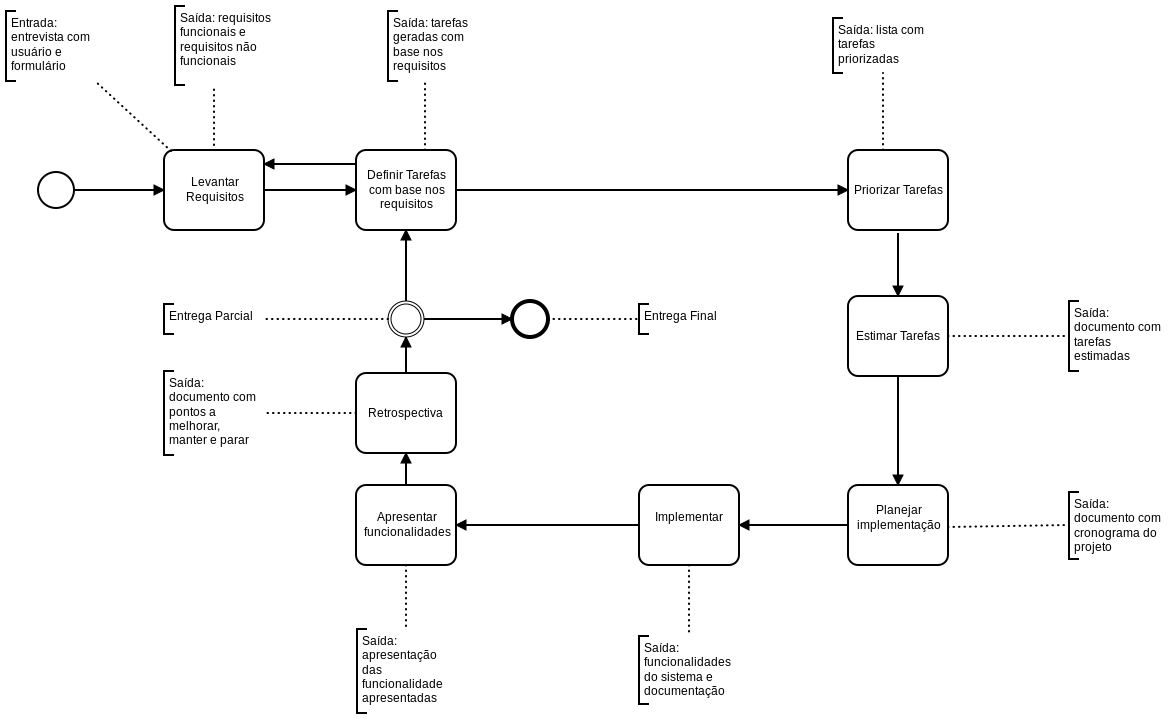
\includegraphics[width=\textwidth]{bpmn.png}
	\caption{BPMN do processo}
	\label{bpmn}
\end{figure}

O processo se inicia com o levantamento de requisitos, onde é feito uma entrevista com o cliente para identificar suas necessidades e transformá-las em atividades que sejam solucionáveis de forma computacional, a partir da entrevista é registrado as histórias de usuário onde, então, será gerado as atividades para a construção do sistema. 

Após a definição das atividades, estas serão priorizadas de acordo as necessidades do cliente e dependências de outras atividades. 

Uma vez que as atividades forem priorizadas, algumas serão selecionadas para que caibam em um período de execução pré-estabelecido, então, segue-se com a reunião de planejamento onde será definido o que é necessário fazer em cada uma das tarefas, assim, a equipe de desenvolvimento já poderá estimar cada uma das tarefas de acordo com a base histórica.

Uma vez que as atividades que foram estimadas caibam na execução da iteração segue-se com a implementação das atividades. Durante a implementação também será escrito os test cases, que serão executados, e também deve ser documentado a funcionalidade que será entregue.Ao final da apresentação deve-se realizar uma apresentação das funcionalidades implementadas ao cliente e preenchido a base histórica. 

Após a apresentação toda a equipe irá fazer uma retrospectiva e apontar os pontos que precisam, melhorar, parar e manter. Após a retrospectiva será entregue uma versão funcional do sistema ao cliente e então o processo se reinicia a até ser entregue a versão final do sistema.


\subsection{Papeis}
\begin{itemize}
	\item Cliente: Define os requisitos do produto que será produzido pelo processo, o que é importante(prioridades/\textit{"key features"}) no produto de software.
	\item Analista de Software: Levantar requisitos claros e concisos, verificar por conflitos, define o  escopo de sistemas novos e como será as modificações nos sistemas já existentes.
	\item Desenvolvedor: Responsável por transformar requisitos e modelos de software em códigos "buildáveis" em determinada linguagem, documentar e descrever cada versão gerada.
	\item Gerente de Projetos: Acompanha a execução do projeto, resolve conflitos, deve acompanhar e gerar artefatos que sustentem a produção de software seguindo requisitos de priorizando a qualidade.
	\item Desenvolvedor \textit{tester}(Opcional): São desenvolvedores que produzem testes baseados nos requisitos, ajudam o gerente a gerar métricas de qualidade de software quantitativas e qualitativas.   
\end{itemize}

\subsection{Atividades}

\begin{enumerate}
	\item \textbf{Levantamento de requisitos}
	\subitem Artefatos de entrada: Questionário e perguntas dissertativas pré-estabelecidas
	\subitem Descrição: O analista de software registra o dialogo com o cliente, faz anotações e usa um questionário padronizado para levantar as funcionalidades e características juntamente com uma descrição delas e do software final, com o cliente, o analista também tenta perceber se existe conflitos, inviabilidade e/ou impossibilidades nos requisitos descritos até então.
	\subitem Artefatos de saída: Formulários de requisitos funcionais e não funcionais preenchido, Questionário respondido 
		
	\item \textbf{Definir tarefas com base nos requisitos}
	\subitem Artefatos de entrada: Formulários de requisitos funcionais e não funcionais
	\subitem Descrição: Com base nos requisitos e anotações anteriores o analista e os desenvolvedores analisam os requisitos e tentam quebra-los em tarefas necessárias para entregar essas funcionalidades.
	\subitem Artefatos de saída: Documento com definição das tarefas e/ou Modelagem

	\item \textbf{Priorizar tarefas} 
	\subitem Artefatos de entrada: Documento com definição das tarefas
	\subitem Descrição: 
	Após tarefas estabelecidas, cabe ao gerente de projeto juntamente com o cliente definir as prioridades de desenvolvimento.
	\subitem Artefatos de saída: Documento definindo um grau de prioridade para cada tarefa e/ou Modelagem
	
		\item \textbf{Estimar Tarefas}  
	\subitem Artefatos de entrada: Base histórica(quando houver), Documento de tarefas
	\subitem Descrição: A estimativa das tarefas são estabelecidas de acordo com o tempo em que serão executada (Utilizando base histórica). Com base na prioridade das tarefas e nas dependências, os desenvolvedores e analista determinam quais serão executadas de acordo com uma sequência estipulada. 
	\subitem Artefatos de saída: Documento definindo tarefas que serão feitas por iteração e/ou Modelagem
	
	
	\item \textbf{Planejar implementação}
	\subitem Artefatos de entrada: Documento definindo tarefas por interação
	\subitem Descrição: 
	A reunião é descrito o que precisa ser feito em cada tarefa e deve ser realizado um protótipo, caso necessário.
	\subitem Artefatos de saída: Documento de proposta de reunião e/ou Modelagem
	
	
	\item \textbf{Implementação}
	\subitem Artefatos de entrada: Documento de requisitos, documento de tarefas da iteração  e/ou Modelagem.
	\subitem Descrição: Nesta fase é o momento em que desenvolvedor elabora o que na atividade estipulado. Caso não exista tester, cada desenvolvedor precisa escrever um test case para sua tarefa e outro desenvolvedor deve testa-la. Documentar cada funcionalidade gerada a partir das tarefas entregues.
	\subitem Artefatos de saída: Linhas de código, Build, Documentações 
	
	\item \textbf{Apresentar Funcionalidades} 
	\subitem Artefatos de entrada: Linhas de código e/ou build.
	\subitem Descrição: É uma reunião onde serão exibidos os "produtos" gerados pela iteração. 
	\subitem Artefatos de saída: \textit{build} do software e documento descrevendo os requisitos implementados. 

	\item \textbf{Retrospectiva} 
	\subitem Artefatos de entrada: Check list de qualidade
	\subitem Descrição: Uma reunião é realizada de modo que apresente os resultados do produto e como foi realizado a sua evolução, focando principalmente em pontos que podem ser melhorados. Cada reunião deve ser preparada antecipadamente de preferência
	\subitem Artefatos de saída: Check list preenchido, conclusão de reunião
\end{enumerate}


\section{Execução do projeto}

Relacione as atividades com os integrantes, crie um cronograma conforme orientações

\subsection{Backlog e sprints}
Backlog 1:
\begin{table}[H]
	\begin{tabular}{|l|l|
		}
		Atividade                               & Stakeholder(s)                                 \\
		Levantamento de Requisitos              & Analista de software, Cliente                  \\
		Definir tarefas com base nos requisitos & Analista e Desenvolvedores                     \\
		Priorizar tarefas                       & Cliente e Gerente de Projeto                   \\
		Estimar tarefas                         & Analista e Desenvolvedores                     \\
		Planejar Implementação                  & Desenvolvedores, Analista e Gerente de Projeto \\
		Implementar                             & Desenvolvedores                                \\
		Apresentar Funcionalidades              & Todos                                          \\
		Retrospectiva                           & Equipe do projeto                             
	\end{tabular}
\end{table}


\subsection{Estado atual}
Artefatos gerados em ordem cronológica, conforme processo. 
\begin{enumerate}
	\item Questionário base (Figura \ref{Figura 2})
	\item Documentos de requisitos funcionais e não funcionais (Figura \ref{Figura 3})
	\item Documento de definição de tarefas e de priorização(Figura \ref{Figura 4})
	\item Artefatos de modelagem(Pode ser feito a partir da documentação dos requisitos)
	\item Documento de planejamento e implantação (Figura \ref{Figura 5})
	\item Documento de Planejamento de implementação (Figuras \ref{Figura 6} \& \ref{Figura 7})
	\item Documento de Prioridades  (Figura \ref{Figura 8})
	\item Linhas de códigos, documentação e/ou build
	\item Documento de Retrospectiva(Geração de histórico)  (Figura \ref{Figura 9})
	\item Documento de Avaliação do cliente  (Figura \ref{Figura 10})
\end{enumerate}


\begin{figure}
	\centering
	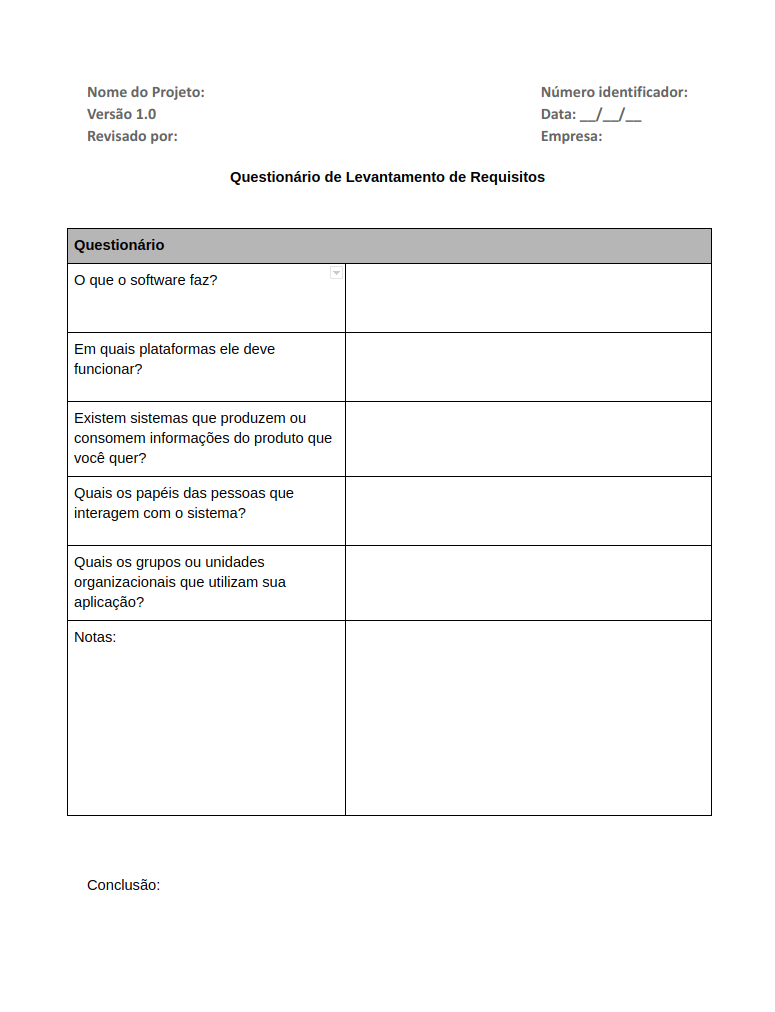
\includegraphics[width=\textwidth]{1.png}
	\caption{Questionário para levantamento de requisitos}
	\label{Figura 1}
\end{figure}

\begin{figure}
	\centering
	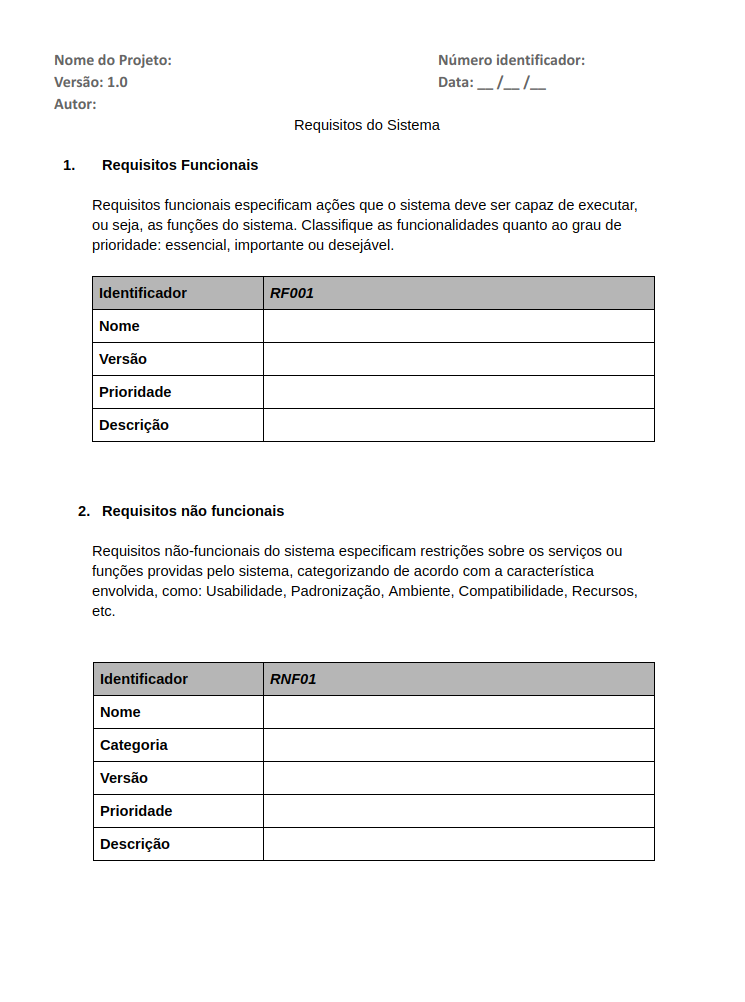
\includegraphics[width=\textwidth]{2.png}
	\caption{Formulário requisitos do sistema}
	\label{Figura 2}
\end{figure}

\begin{figure}
	\centering
	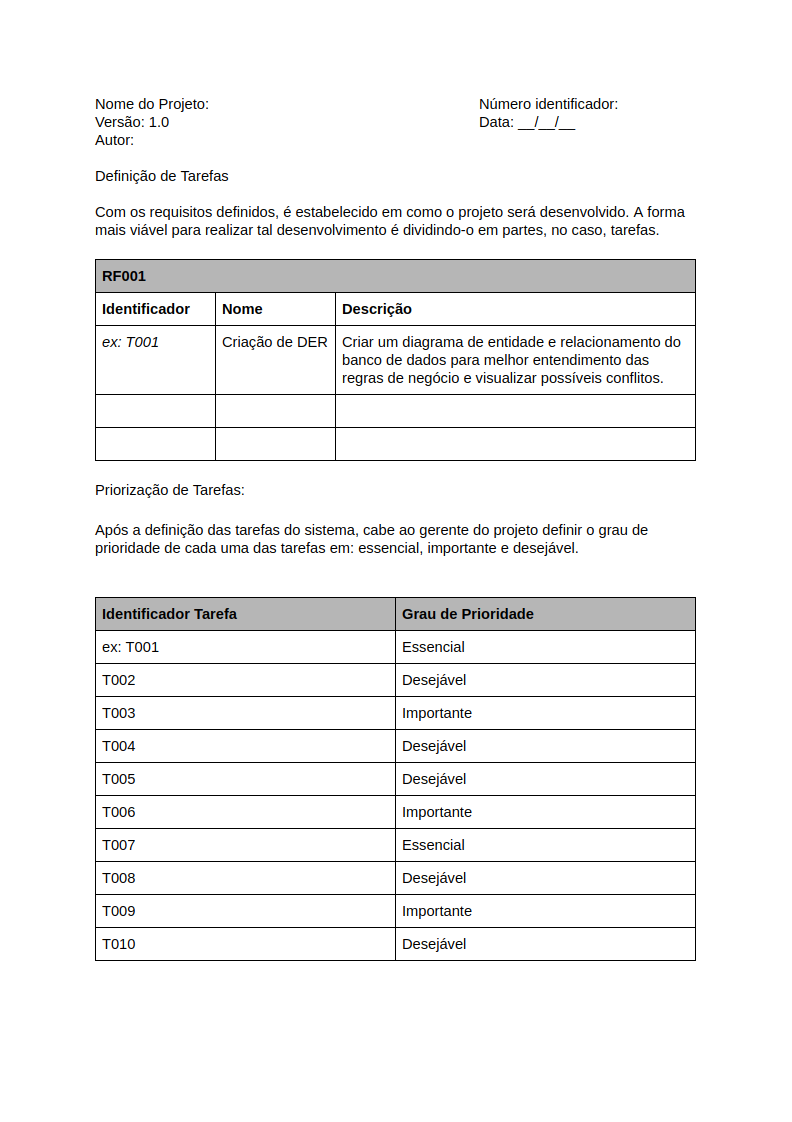
\includegraphics[width=\textwidth]{3.png}
	\caption{Definição de tarefas e prioridades}
	\label{Figura 3}
\end{figure}


\begin{figure}
	\centering
	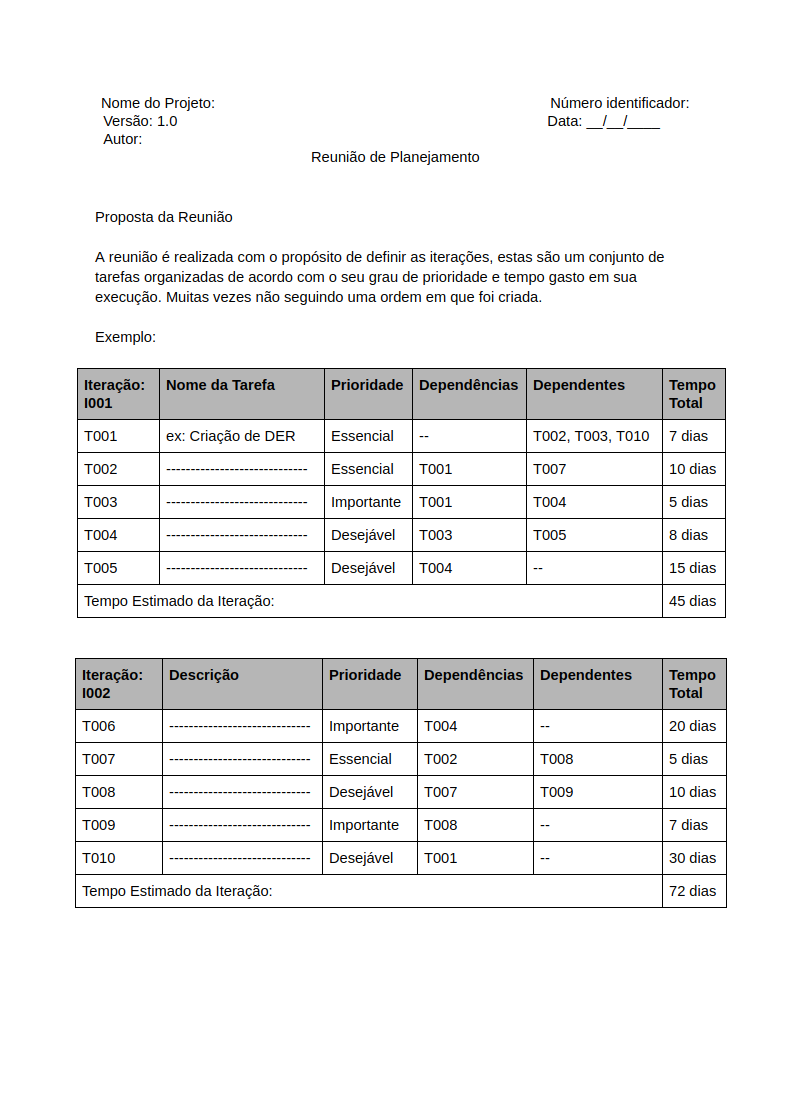
\includegraphics[width=\textwidth]{4-1.png}
	\caption{Planejamento da implementação}
	\label{Figura 4}
\end{figure}


\begin{figure}
	\centering
	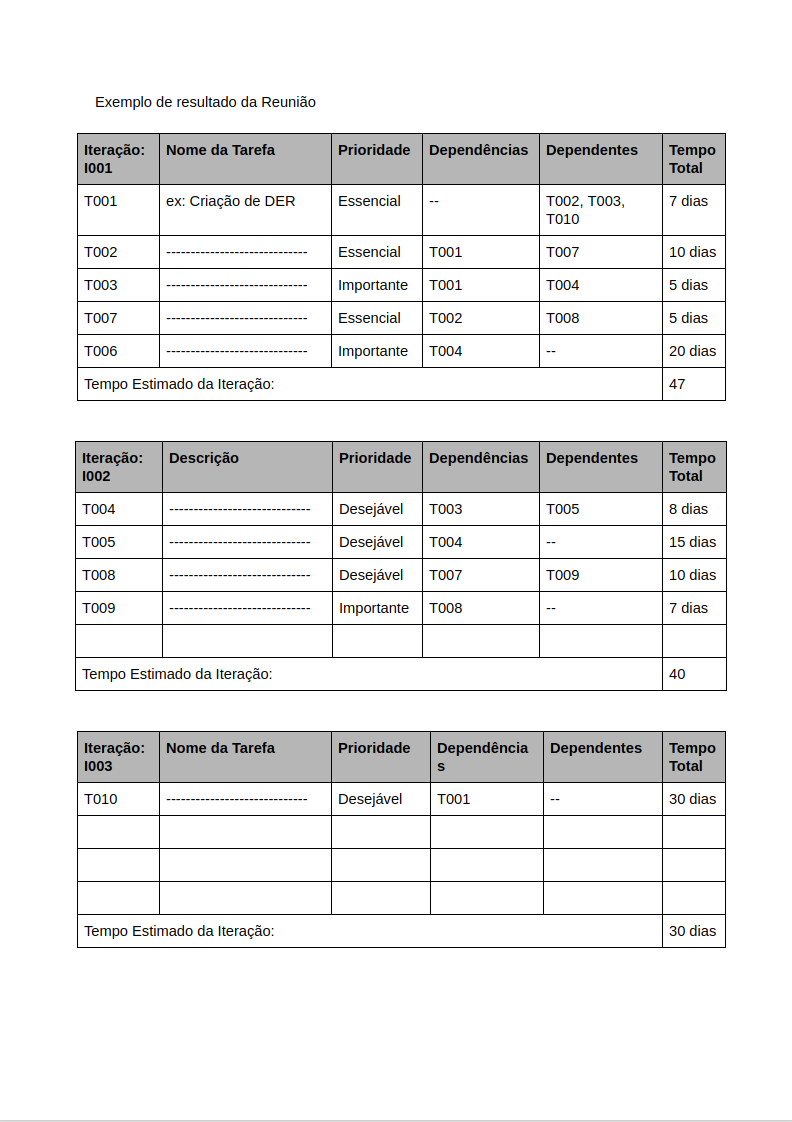
\includegraphics[width=\textwidth]{4-2.png}
	\caption{Planejamento da implementação}
	\label{Figura 5}
\end{figure}

\begin{figure}
	\centering
	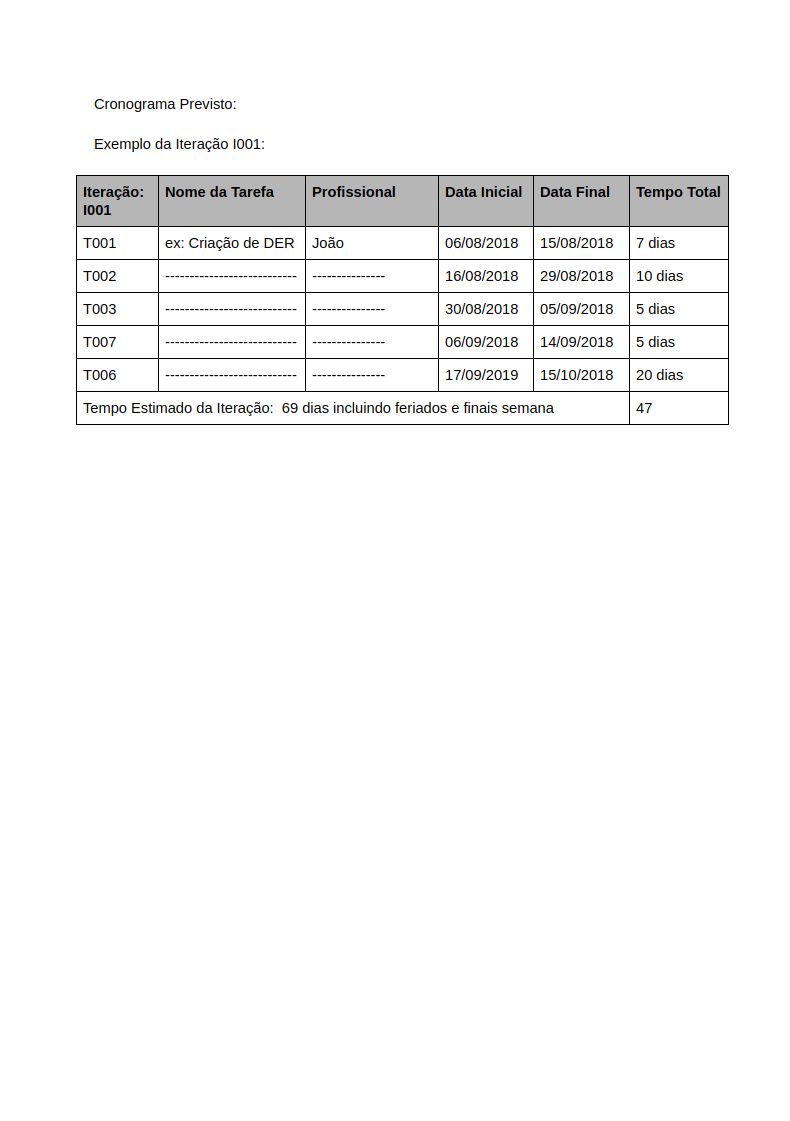
\includegraphics[width=\textwidth]{4-3.png}
	\caption{Planejamento da implementação}
	\label{Figura 6}
\end{figure}

\begin{figure}
	\centering
	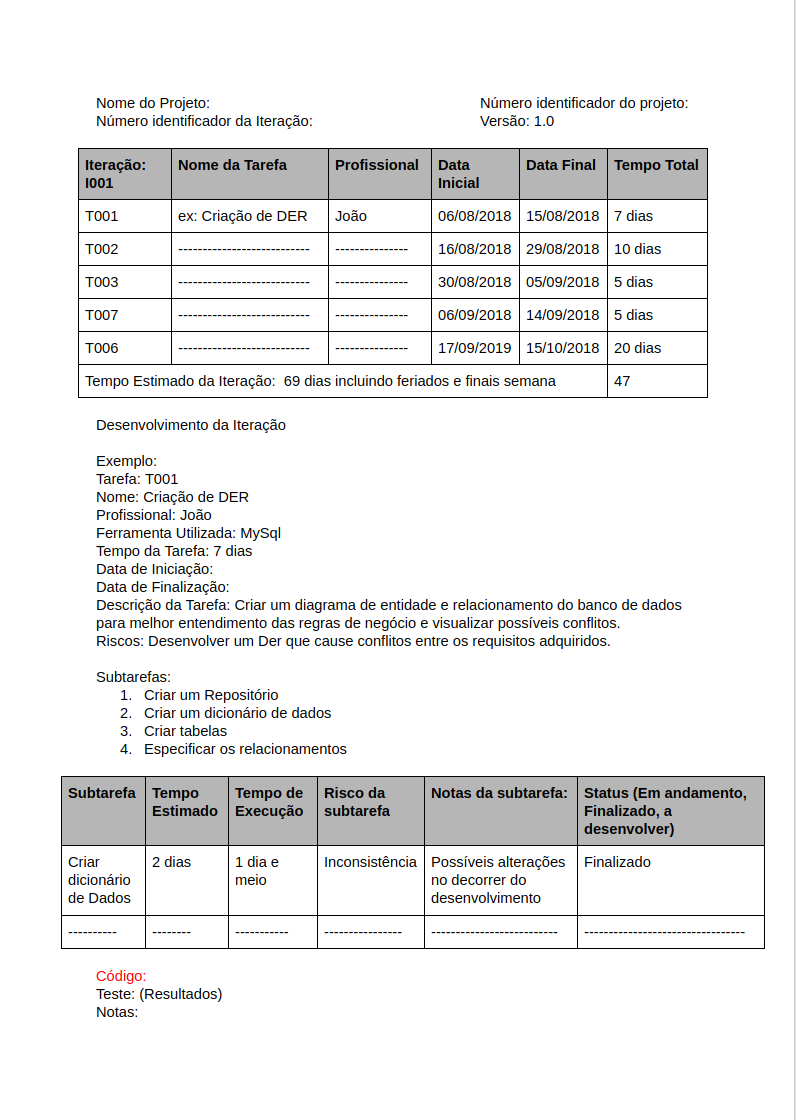
\includegraphics[width=\textwidth]{5.png}
	\caption{Exemplo de iteração}
	\label{Figura 7}
\end{figure}


\begin{figure}
	\centering
	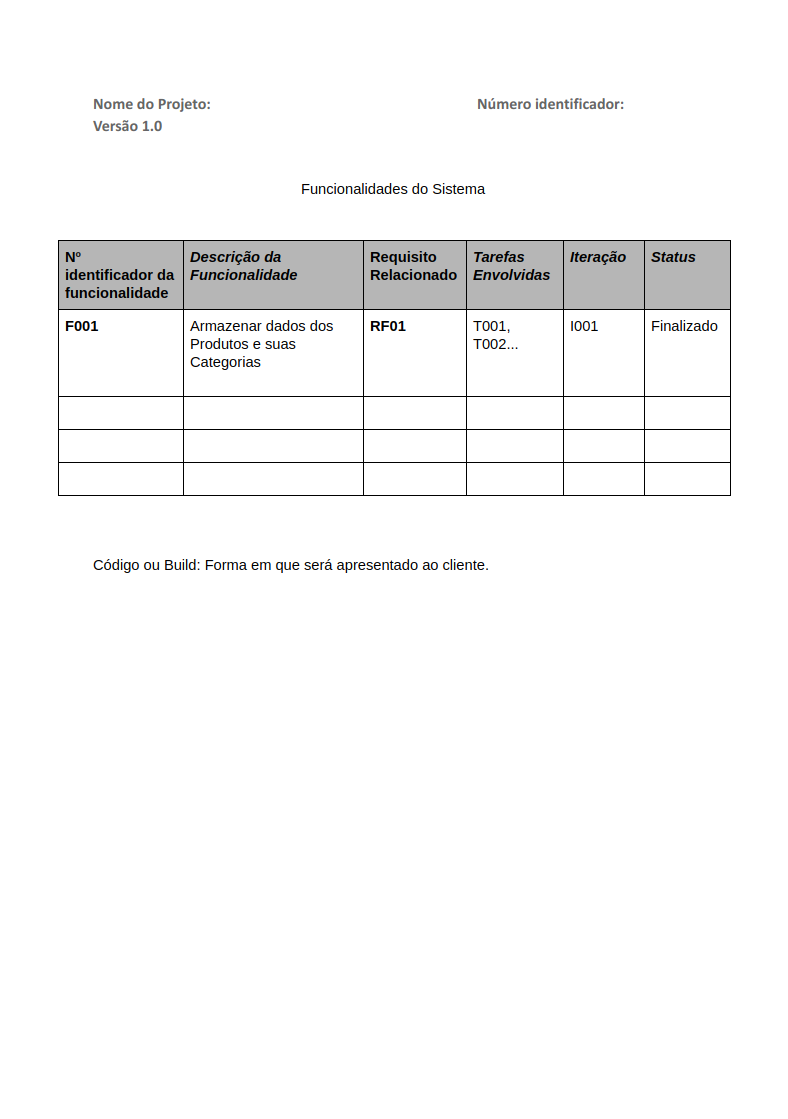
\includegraphics[width=\textwidth]{6.png}
	\caption{Funcionalidades}
	\label{Figura 8}
\end{figure}



\begin{figure}
	\centering
	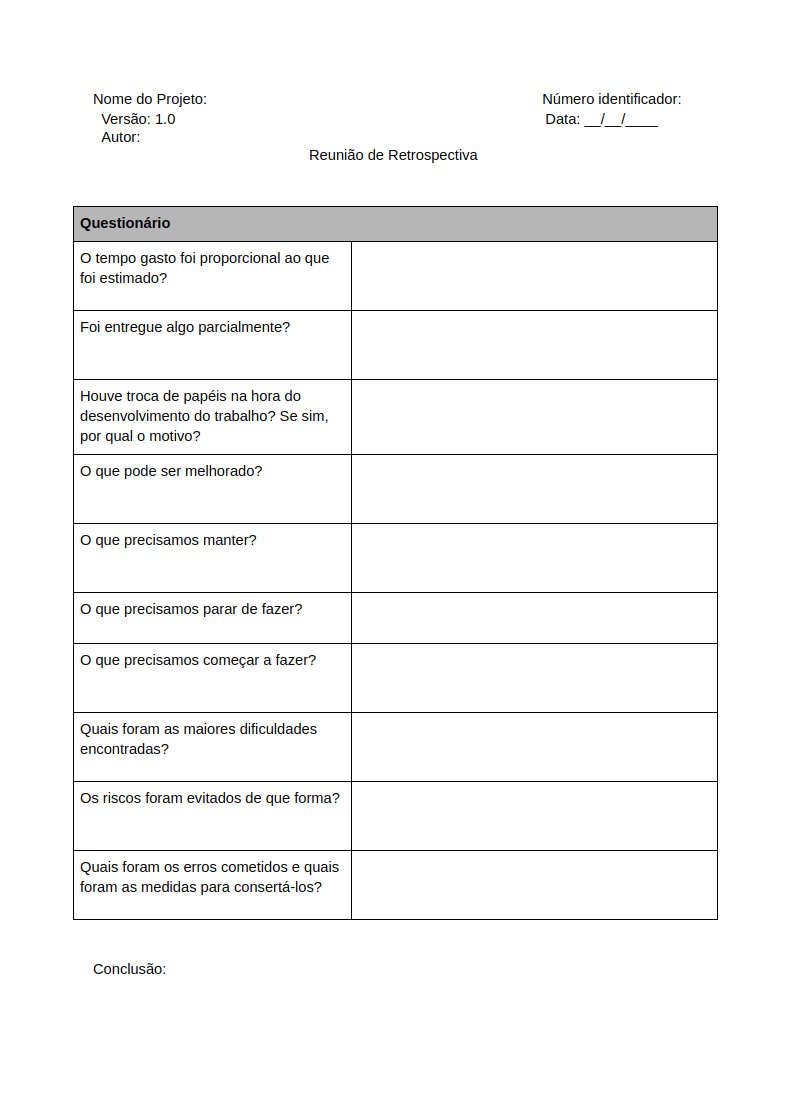
\includegraphics[width=\textwidth]{7.png}
	\caption{Retrospectiva}
	\label{Figura 9}
\end{figure}

\begin{figure}
	\centering
	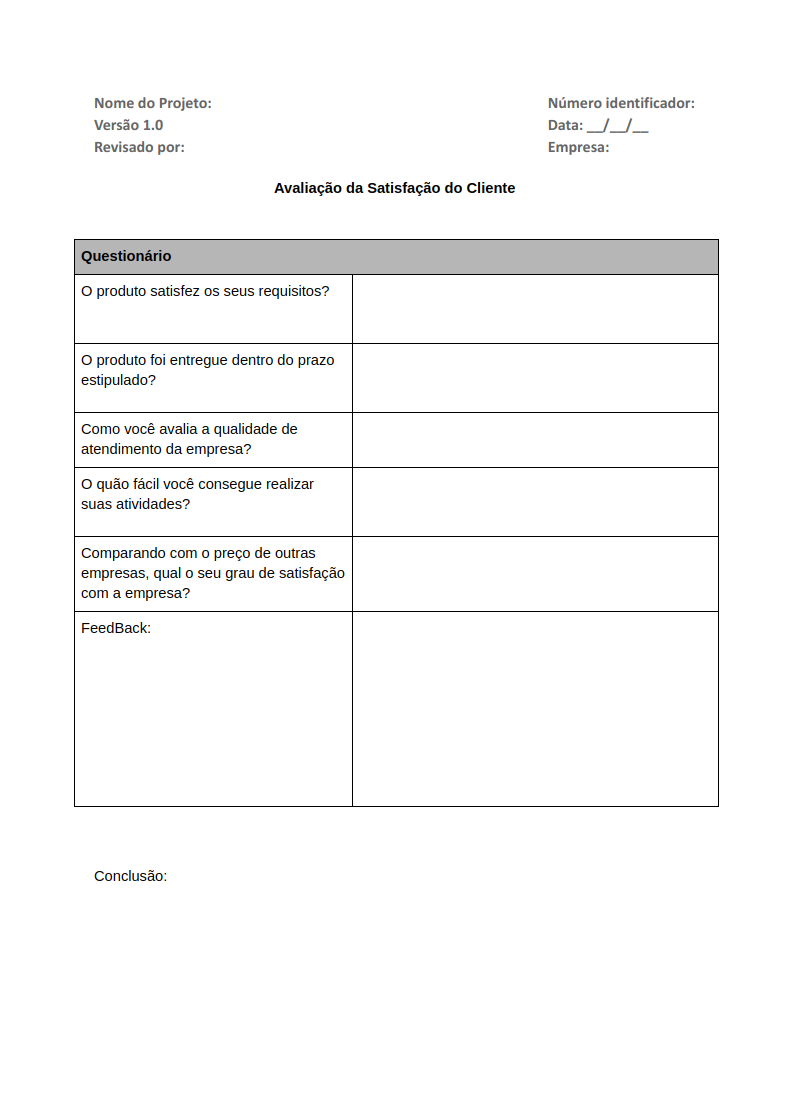
\includegraphics[width=\textwidth]{8.png}
	\caption{Avaliação do cliente}
	\label{Figura 10}
\end{figure}





\section{Referências bibliográficas}
\renewcommand\refname{} %%Referências bibliográficas}  
\bibliographystyle{ieeetr}
\bibliography{referencias} 
\end{document}